% !TEX program = xelatex
\documentclass[11pt,a4paper]{article}

% ---------- Ngôn ngữ & Mã hóa ----------
\usepackage{fontspec}
\usepackage{polyglossia}
\setdefaultlanguage{vietnamese}

% Font hỗ trợ tiếng Việt (dùng Noto Sans — có đầy đủ glyph tiếng Việt)
\setmainfont{Noto Sans}
\setsansfont{Noto Sans}
\setmonofont{Noto Sans Mono}

% ---------- Cấu trúc ----------
\usepackage{titlesec}
\usepackage{geometry}
\geometry{a4paper, top=1.8cm, bottom=1.8cm, left=2cm, right=2cm}
\setlength{\parindent}{0pt}
\setlength{\parskip}{3pt}
\linespread{1.1}   % dòng đều đặn, không giãn quá mức
\emergencystretch=3em

% ---------- Bảng ----------
\usepackage{booktabs}
\usepackage{array}
\usepackage{longtable}
\usepackage{colortbl}
\renewcommand{\arraystretch}{1.12}
\usepackage{tabularx}
\newcolumntype{L}[1]{>{\raggedright\arraybackslash}p{#1}}

% ---------- Đồ họa ----------
\usepackage{graphicx}
\usepackage{float}
\usepackage{caption}
\captionsetup{font=small,skip=3pt}
\graphicspath{{assets/}}

% ---------- Code (môi trường listing) ----------
\usepackage{xcolor}
\definecolor{codebg}{RGB}{245,245,245}
\definecolor{codeframe}{RGB}{220,220,220}
\definecolor{commentcolor}{RGB}{106,153,85}
\definecolor{keywordcolor}{RGB}{0,0,255}
\definecolor{stringcolor}{RGB}{163,21,21}
\definecolor{verbbg}{RGB}{248,248,248}
\usepackage{listings}
\lstset{
  basicstyle=\ttfamily\small,
  backgroundcolor=\color{verbbg},
  frame=single,
  rulecolor=\color{codeframe},
  breaklines=true,
  showstringspaces=false,
  commentstyle=\color{commentcolor},
  keywordstyle=\color{keywordcolor},
  stringstyle=\color{stringcolor},
  aboveskip=4pt,
  belowskip=4pt,
}

% Ký hiệu check/cross
\usepackage{amssymb}
\usepackage{pifont}

% Inline code dùng \ccode{...}
\usepackage{etoolbox}
\usepackage{amsfonts}
\newcommand{\ccode}[1]{\texttt{\small #1}}
% Đường dẫn ngắt dòng được (không tràn lề)
\usepackage{url}
\urlstyle{tt}
\def\UrlBreaks{\do\/\do\-}   % cho phép ngắt dòng tại / và -
\newcommand{\cpath}[1]{\small\path{#1}}

% ---------- Siêu liên kết ----------
\usepackage[hidelinks]{hyperref}
\usepackage[export]{adjustbox}

% ---------- Màu & cỡ tiêu đề ----------
\definecolor{seccolor}{RGB}{0,60,120}
% Giảm khoảng trắng trước/sau heading để tránh lãng phí pagination
\titlespacing*{\section}{0pt}{10pt}{5pt}
\titlespacing*{\subsection}{0pt}{8pt}{3pt}
\titlespacing*{\subsubsection}{0pt}{6pt}{2pt}
\titleformat{\section}
  {\fontsize{16}{18}\bfseries\color{seccolor}}{\thesection}{0.7em}{}
\titleformat{\subsection}
  {\fontsize{13}{15}\bfseries\color{seccolor}}{\thesubsection}{0.7em}{}
\titleformat{\subsubsection}
  {\fontsize{11}{13}\bfseries\color{seccolor}}{\thesubsubsection}{0.7em}{}

\begin{document}

% ============================================================
% 1. Tổng quan
% ============================================================
\section{Tổng quan}

\subsection{CyberStrikeAI là gì?}

CyberStrikeAI là \textbf{nền tảng pentest tự động hóa AI-native} --- kết hợp lập kế hoạch, thực thi, giám sát con người, bằng chứng (evidence), và phân tích trong một workspace có kiểm soát. Hệ thống được xây dựng bằng Go, sử dụng các agent AI để thực hiện các tác vụ bảo mật (reconnaissance, vulnerability analysis, exploitation guidance, reporting).

\textbf{Đặc điểm chính:}
\begin{itemize}
  \item \textbf{Agent-based execution}: AI phân tích yêu cầu, lập kế hoạch, gọi công cụ (tools), và tổng hợp kết quả.
  \item \textbf{Human-in-the-loop (HITL)}: Hỗ trợ phê duyệt trước khi thực thi các công cụ nhạy cảm.
  \item \textbf{Evidence-based}: Mọi kết quả được lưu trữ và liên kết (fact board, assets, vulnerabilities).
  \item \textbf{Modular \& extensible}: Hỗ trợ MCP (Model Context Protocol), skills, roles, workflows.
  \item \textbf{RBAC}: Quản lý người dùng, vai trò, và phân quyền chi tiết.
\end{itemize}

\subsection{Các chức năng chính}

Nền tảng cung cấp chat/agent AI để giao việc và theo dõi thực thi, tổ chức engagement theo \textbf{Project} với chuỗi tấn công (attack chain), quản lý \textbf{Assets} và \textbf{Vulnerabilities} theo dự án, và hỗ trợ các tính năng mở rộng như \textbf{MCP}, \textbf{Knowledge Base}, \textbf{Skills}, \textbf{Roles}, \textbf{Workflows}, cùng ghi log \textbf{Audit} mọi thao tác.

\begin{figure}[htbp]
  \centering
  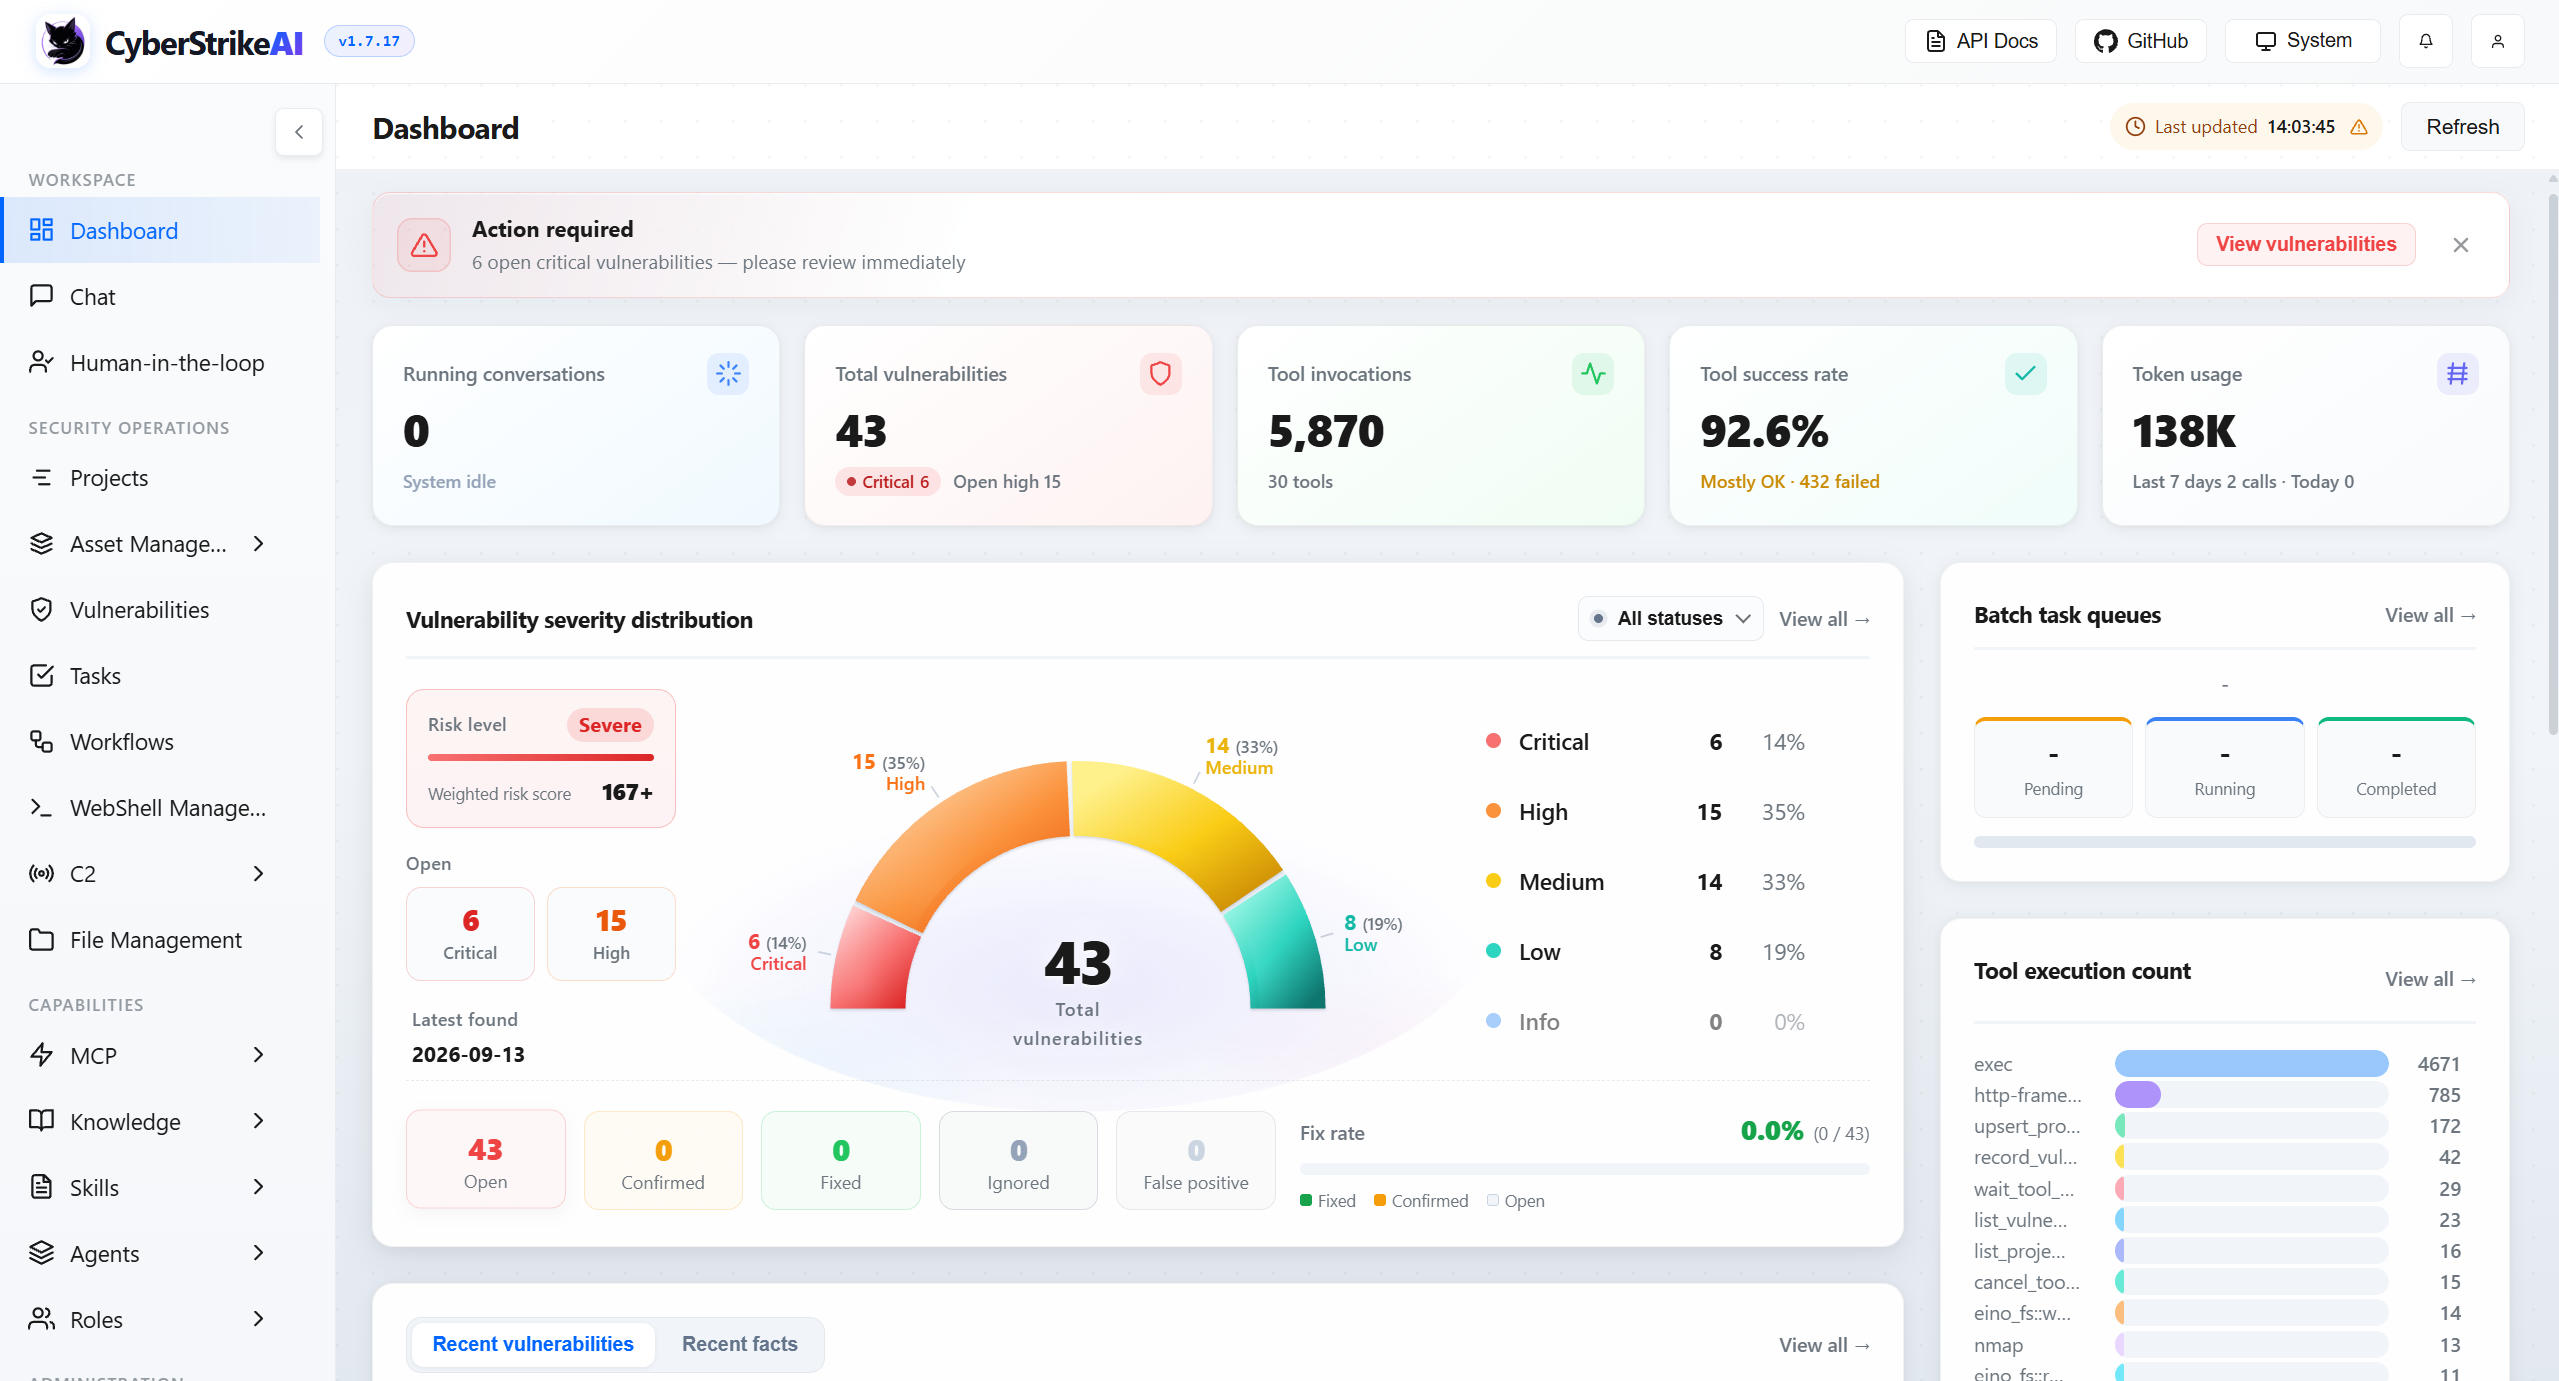
\includegraphics[width=0.78\textwidth,keepaspectratio]{01-dashboard.png}
  \caption{Dashboard overview}
\end{figure}

\subsection{Phạm vi tài liệu}

Tài liệu này hướng dẫn:
\begin{itemize}
  \item[\checkmark] Cài đặt và khởi chạy (local, Docker).
  \item[\checkmark] Cấu hình cơ bản (AI, tools, MCP, HITL).
  \item[\checkmark] Quy trình sử dụng từ tạo project đến quản lý kết quả.
  \item[\checkmark] Troubleshooting các lỗi thường gặp.
\end{itemize}

\textbf{Không đề cập sâu:}
\begin{itemize}
  \item[\ding{55}] C2 (Command \& Control) --- xem \cpath{docs/en-US/c2.md}.
  \item[\ding{55}] WebShell management --- xem \cpath{docs/en-US/webshell.md}.
  \item[\ding{55}] Plugin development (Burp Suite, browser extension) --- xem \cpath{docs/en-US/plugin-development.md}.
\end{itemize}

% ============================================================
% 2. Cài đặt và Cấu hình
% ============================================================
\section{Cài đặt và Cấu hình}

\subsection{Yêu cầu}

\textbf{Docker} 20.10+ \& \textbf{Docker Compose} v2+ (khuyến nghị), hoặc Go 1.21+ \& Python 3.10+ cho chế độ development. Cần \textbf{API key} của một AI provider (OpenAI, DeepSeek, Qwen, Claude, Viettel Netmind) và có thể cài thêm các tool bảo mật (nmap, sqlmap, nuclei, gobuster).

\subsection{Cài đặt với Docker (Khuyến nghị)}

\begin{lstlisting}[language=bash]
# 1. Clone repo
git clone https://github.com/Akapi895/RedForge.git
cd RedForge

# 2. Prepare config + configure AI model (see "Cau hinh AI Model" below)
cp config.example.yaml config.yaml

# 3. Start container (set password first to change default admin123)
export CYBERSTRIKE_ADMIN_PASSWORD=admin123
docker compose up -d --build
docker compose ps
docker compose logs -f
\end{lstlisting}

\begin{figure}[htbp]
  \centering
  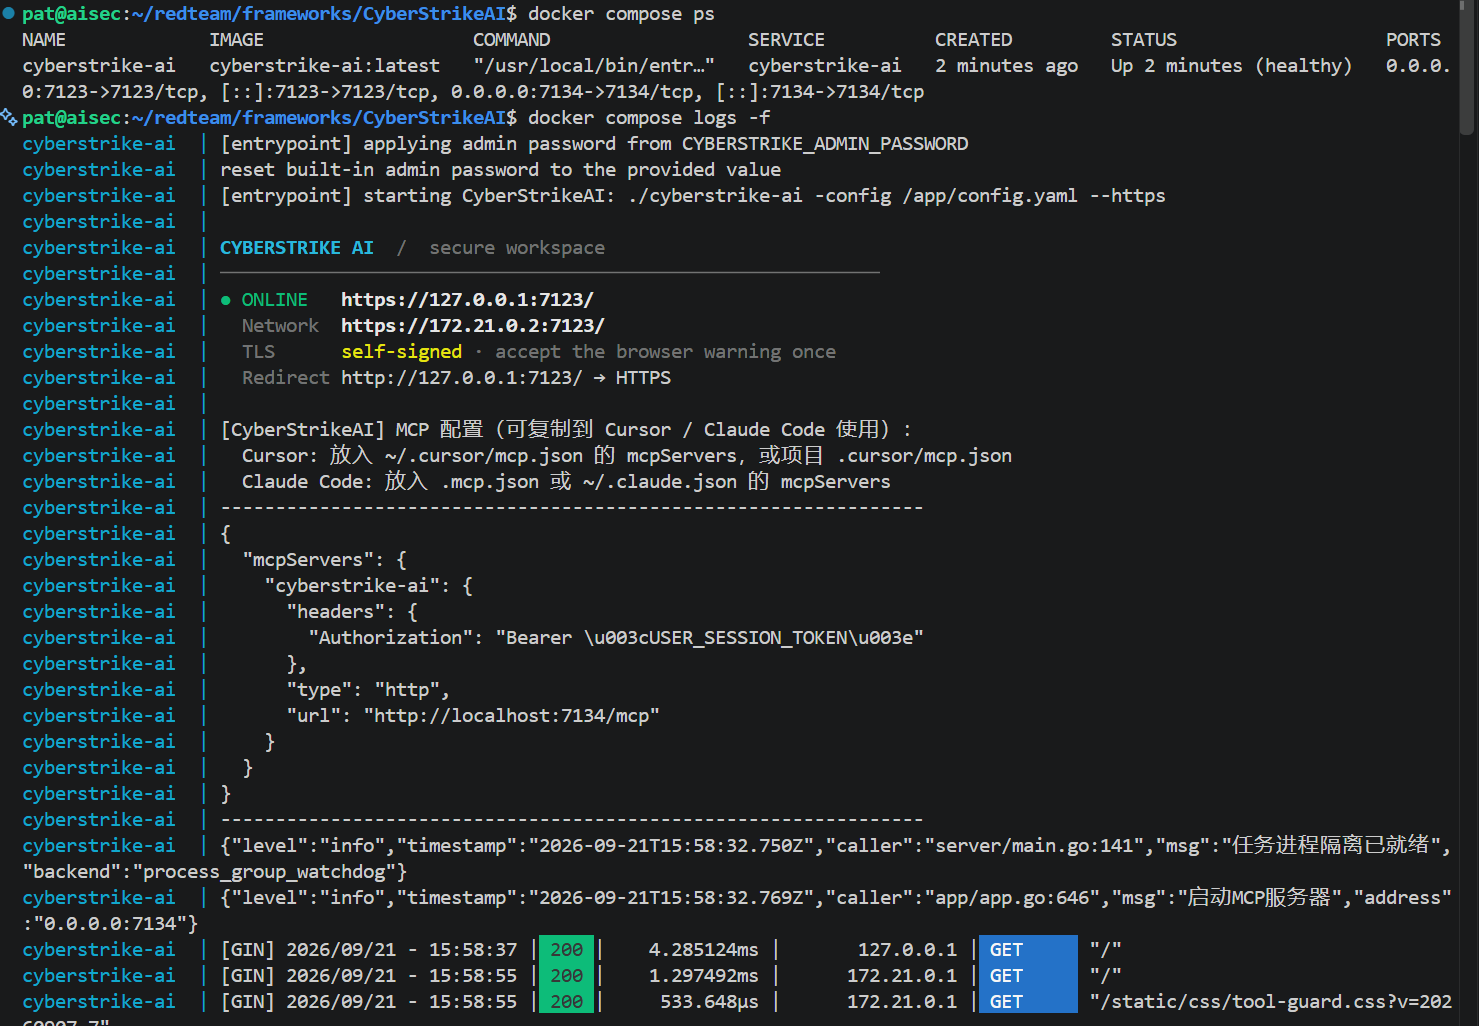
\includegraphics[width=0.66\textwidth,keepaspectratio]{01-docker-ps.png}
  \caption{Docker compose ps}
\end{figure}

\subsection{Cài đặt với run.sh (Development)}

\begin{lstlisting}[language=bash]
go mod download
python3 -m venv venv && source venv/bin/activate
pip install -r requirements.txt
export CYBERSTRIKE_ADMIN_PASSWORD=admin123
chmod +x run.sh && ./run.sh
\end{lstlisting}

Server khởi động trên \textbf{port 7123} (HTTPS) và \textbf{port 7134} (MCP). Truy cập \textbf{\ccode{https://localhost:7123/}}, chấp nhận chứng chỉ tự-signed, đăng nhập \ccode{admin} / \ccode{admin123} (hoặc giá trị bạn set).

\subsection{Cấu hình AI Model}\label{sec:ai-config}

Web UI chỉ hiển thị danh sách AI channels (read-only). Để thêm/sửa channel, mở \ccode{config.yaml}, chỉnh section \ccode{ai.channels}, rồi restart server:

\begin{lstlisting}[]
ai:
  default_channel: netmind
  channels:
    netmind:
      name: Viettel MiniMax M3
      provider: openai_compatible
      base_url: https://stream-netmind.viettel.vn/aigw/ai/v1
      api_key: <sk-your-key>
      model: MiniMax/MiniMax-M3
\end{lstlisting}

\begin{lstlisting}[language=bash]
# Docker
docker compose restart
# Hoac run.sh
Ctrl+C && ./run.sh
\end{lstlisting}

\subsection{Cấu hình Optional (MCP \& HITL)}

\textbf{MCP (Model Context Protocol)} — bật \ccode{mcp.enabled: true} (port mặc định 7134) để kết nối công cụ bên ngoài. Nếu dùng external server, khai báo trong \ccode{external\_mcp.servers} với transport HTTP/stdio và kiểm tra kết nối trong giao diện.

\textbf{Human-in-the-Loop (HITL)} — đặt \ccode{hitl.default\_mode: approval} để yêu cầu phê duyệt trước khi thực thi công cụ nhạy cảm; các tool an toàn có thể nằm trong \ccode{tool\_whitelist}.

\begin{figure}[htbp]
  \centering
  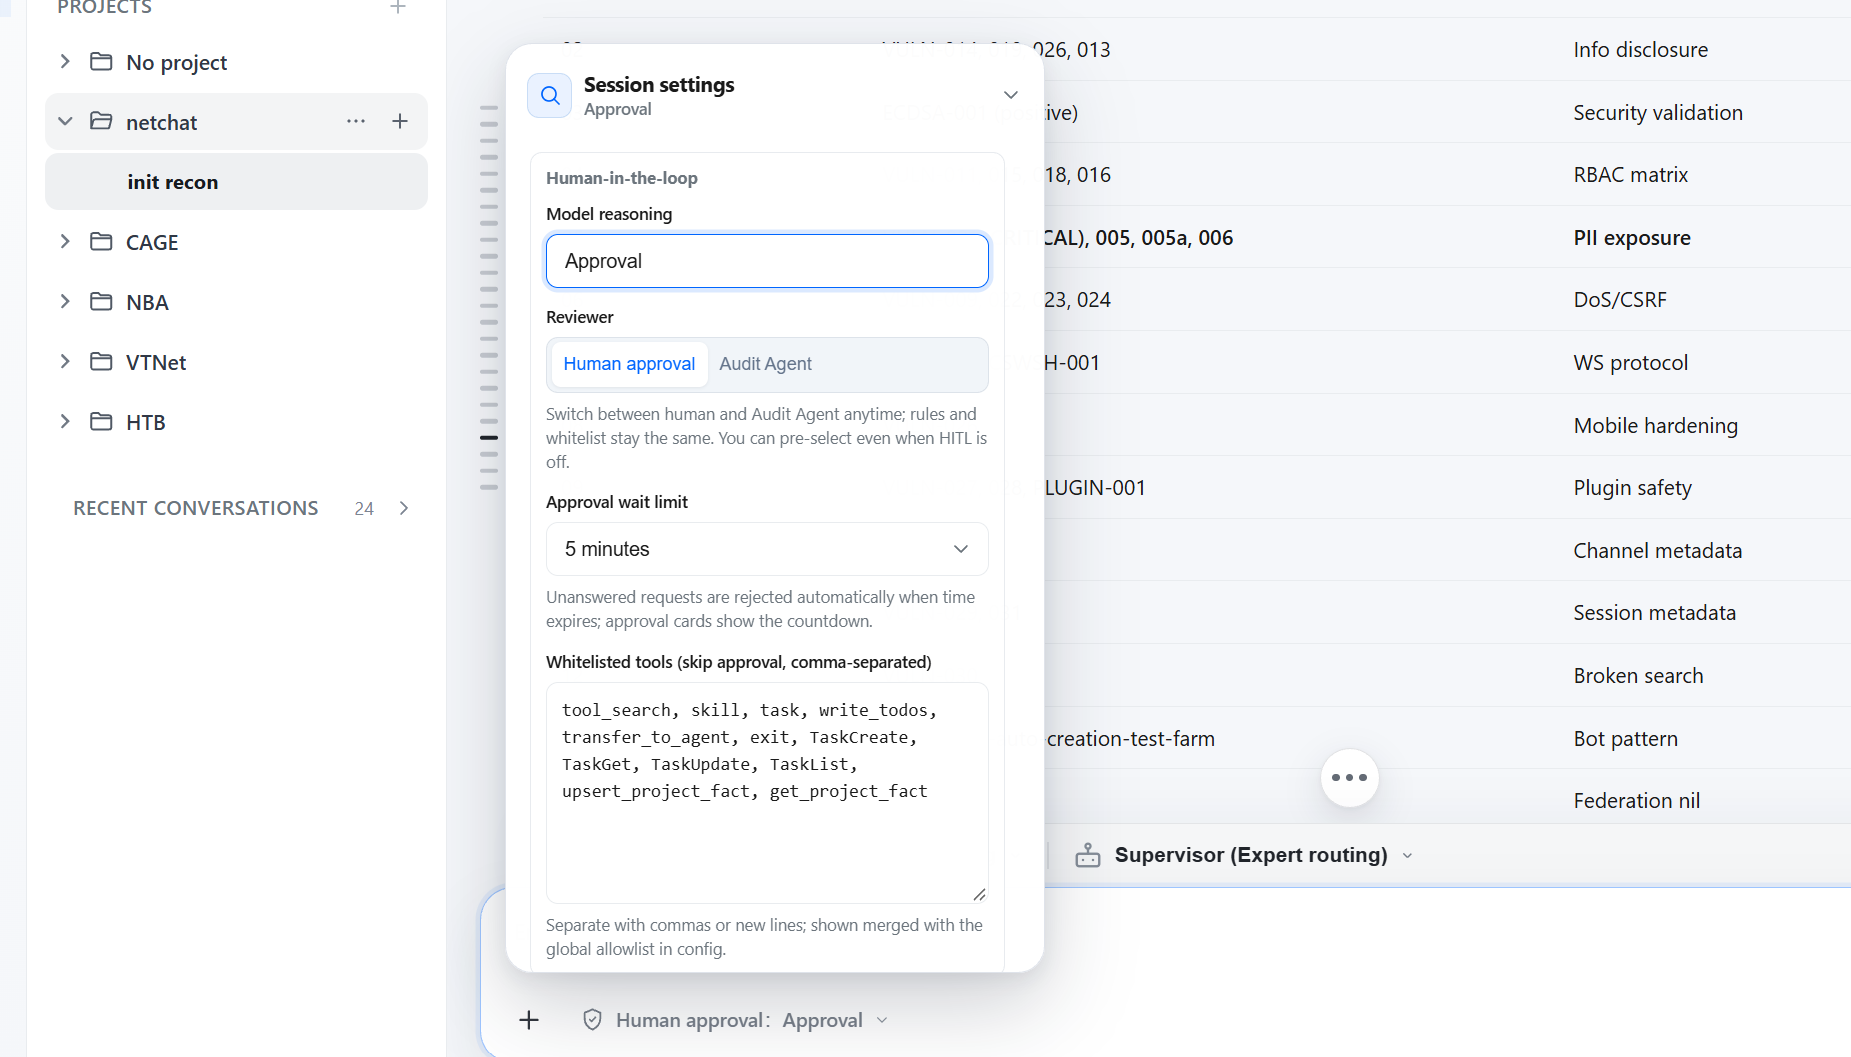
\includegraphics[width=0.66\textwidth,keepaspectratio]{02-hitl.png}
  \caption{HITL configuration}
\end{figure}

% ============================================================
% 3. Quy trình Sử dụng
% ============================================================
\section{Quy trình Sử dụng}

\subsection*{Quy trình hoàn chỉnh}

\subsection{Bước 1: Tạo Project}

Vào \textbf{Projects} $\rightarrow$ \textbf{New Project}, điền \textbf{Name}, \textbf{Description}, \textbf{Scope} (JSON, optional), rồi \textbf{Create}. Project là container gom conversation, fact, asset, vulnerability của cùng một engagement.

\begin{figure}[htbp]
  \centering
  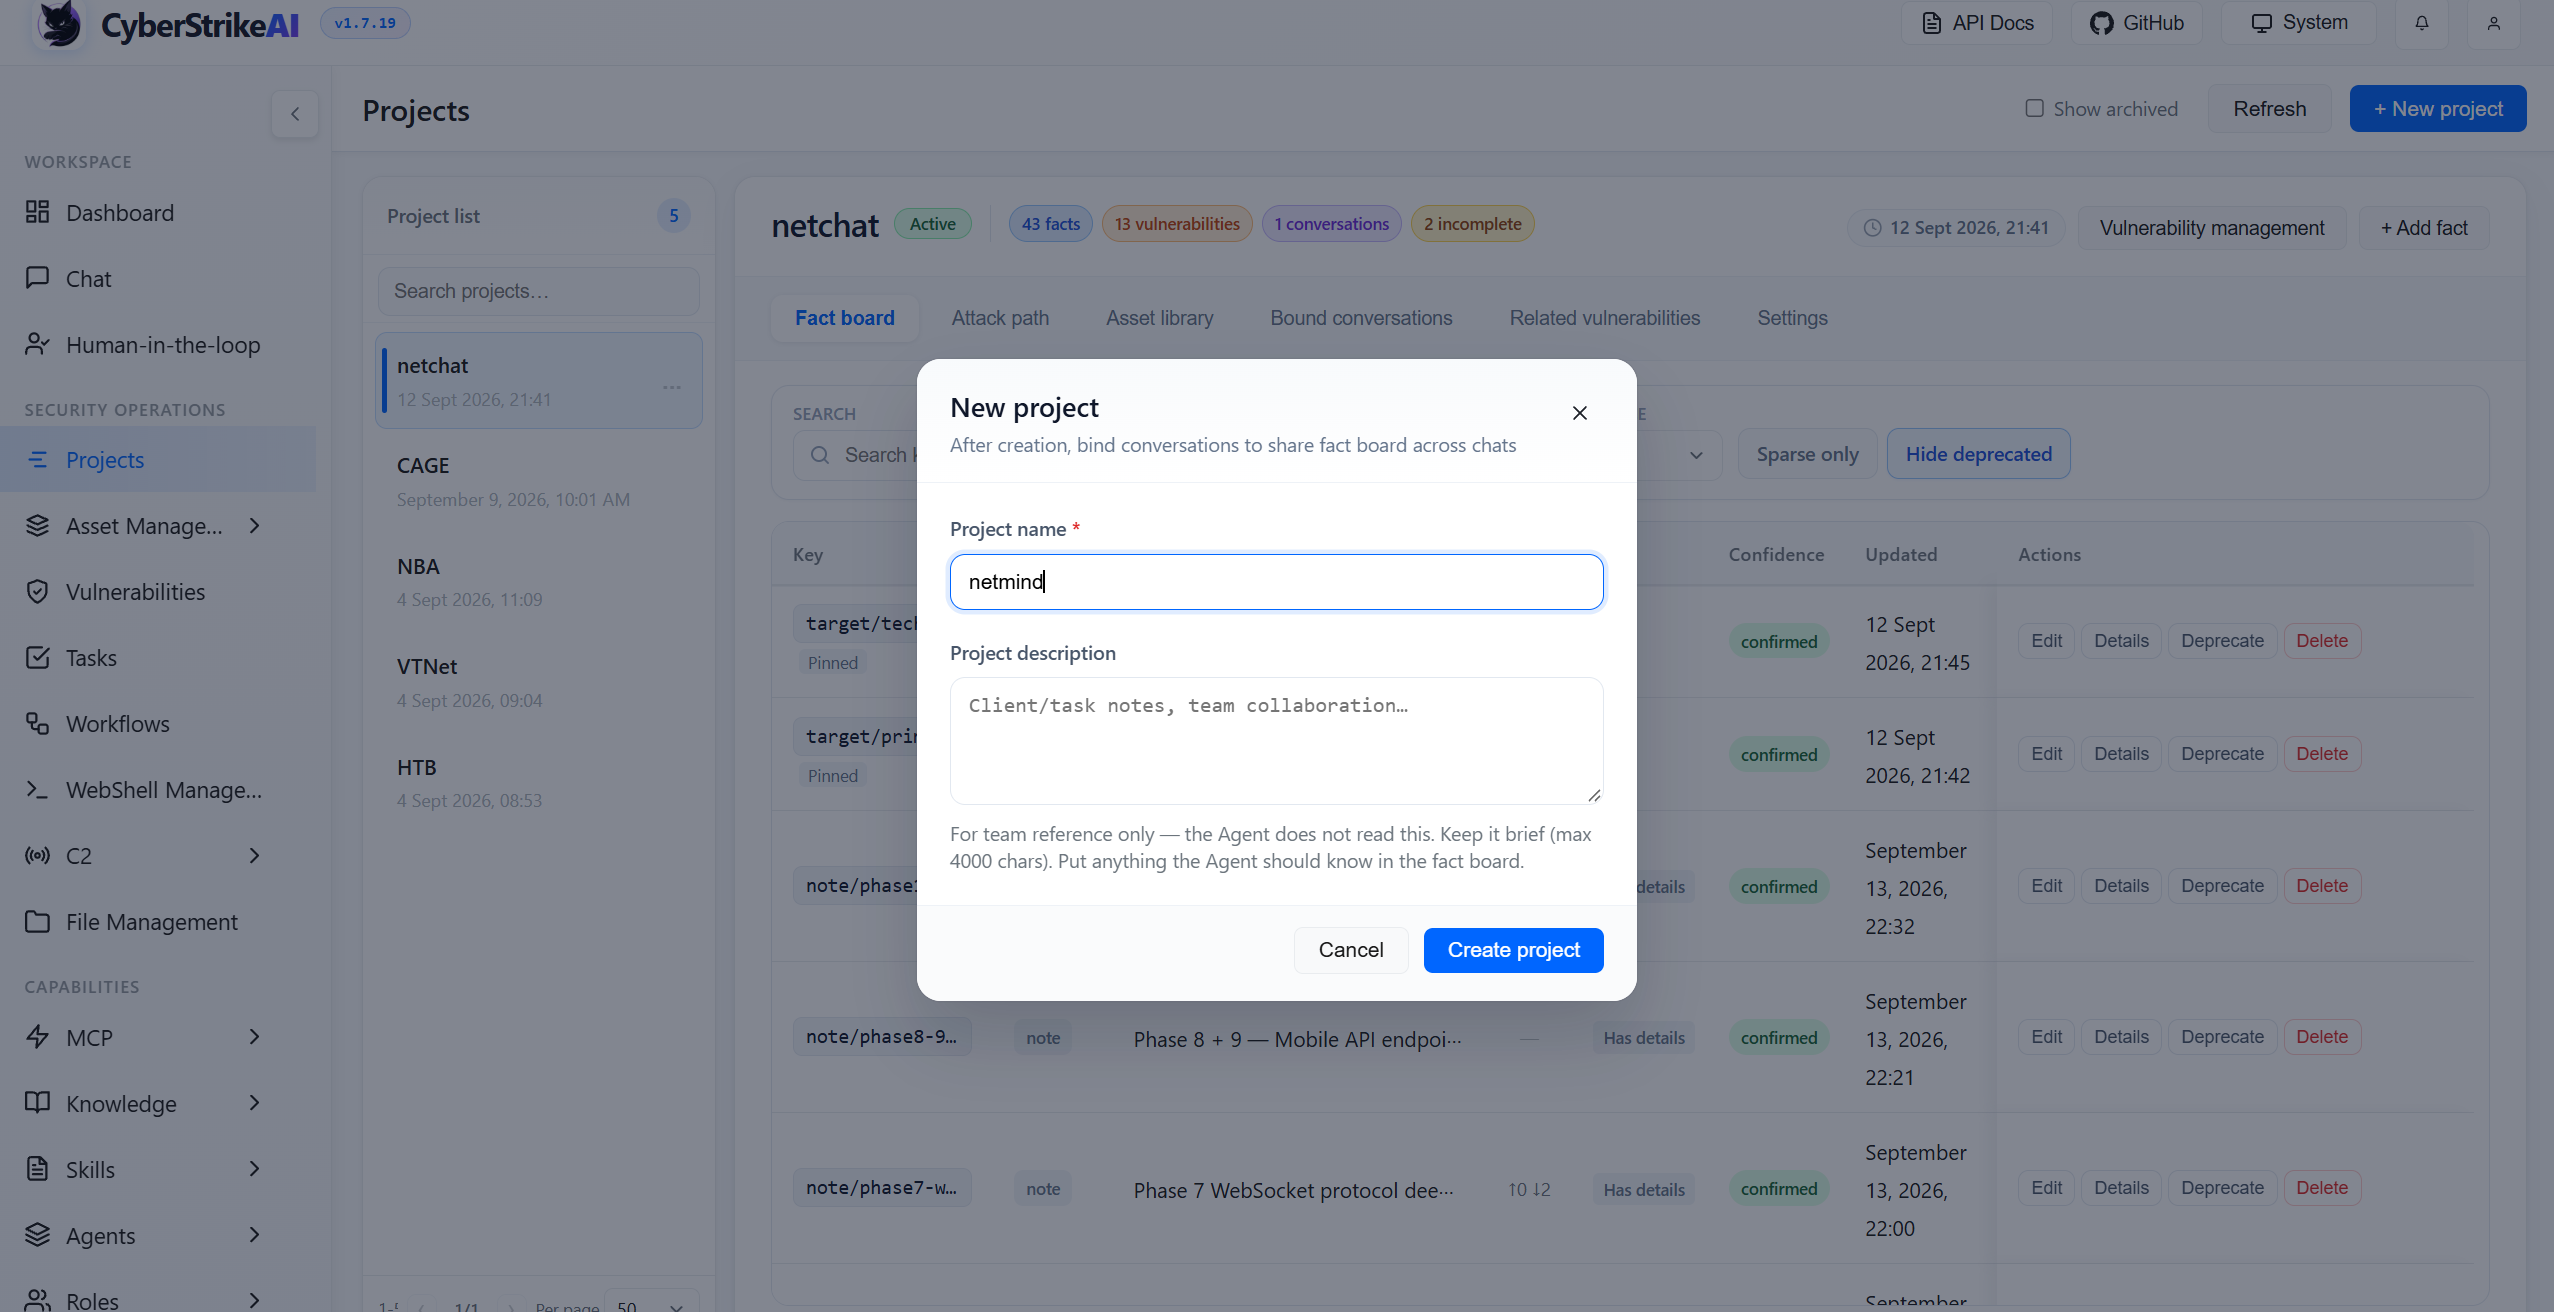
\includegraphics[width=0.66\textwidth,keepaspectratio]{01-new-project.png}
  \caption{New Project form}
\end{figure}

\subsection{Bước 2: Mở Chat}

Vào \textbf{Chat} $\rightarrow$ \textbf{New Conversation} (hoặc chọn project từ dropdown), rồi nhập yêu cầu vào composer.

\begin{figure}[htbp]
  \centering
  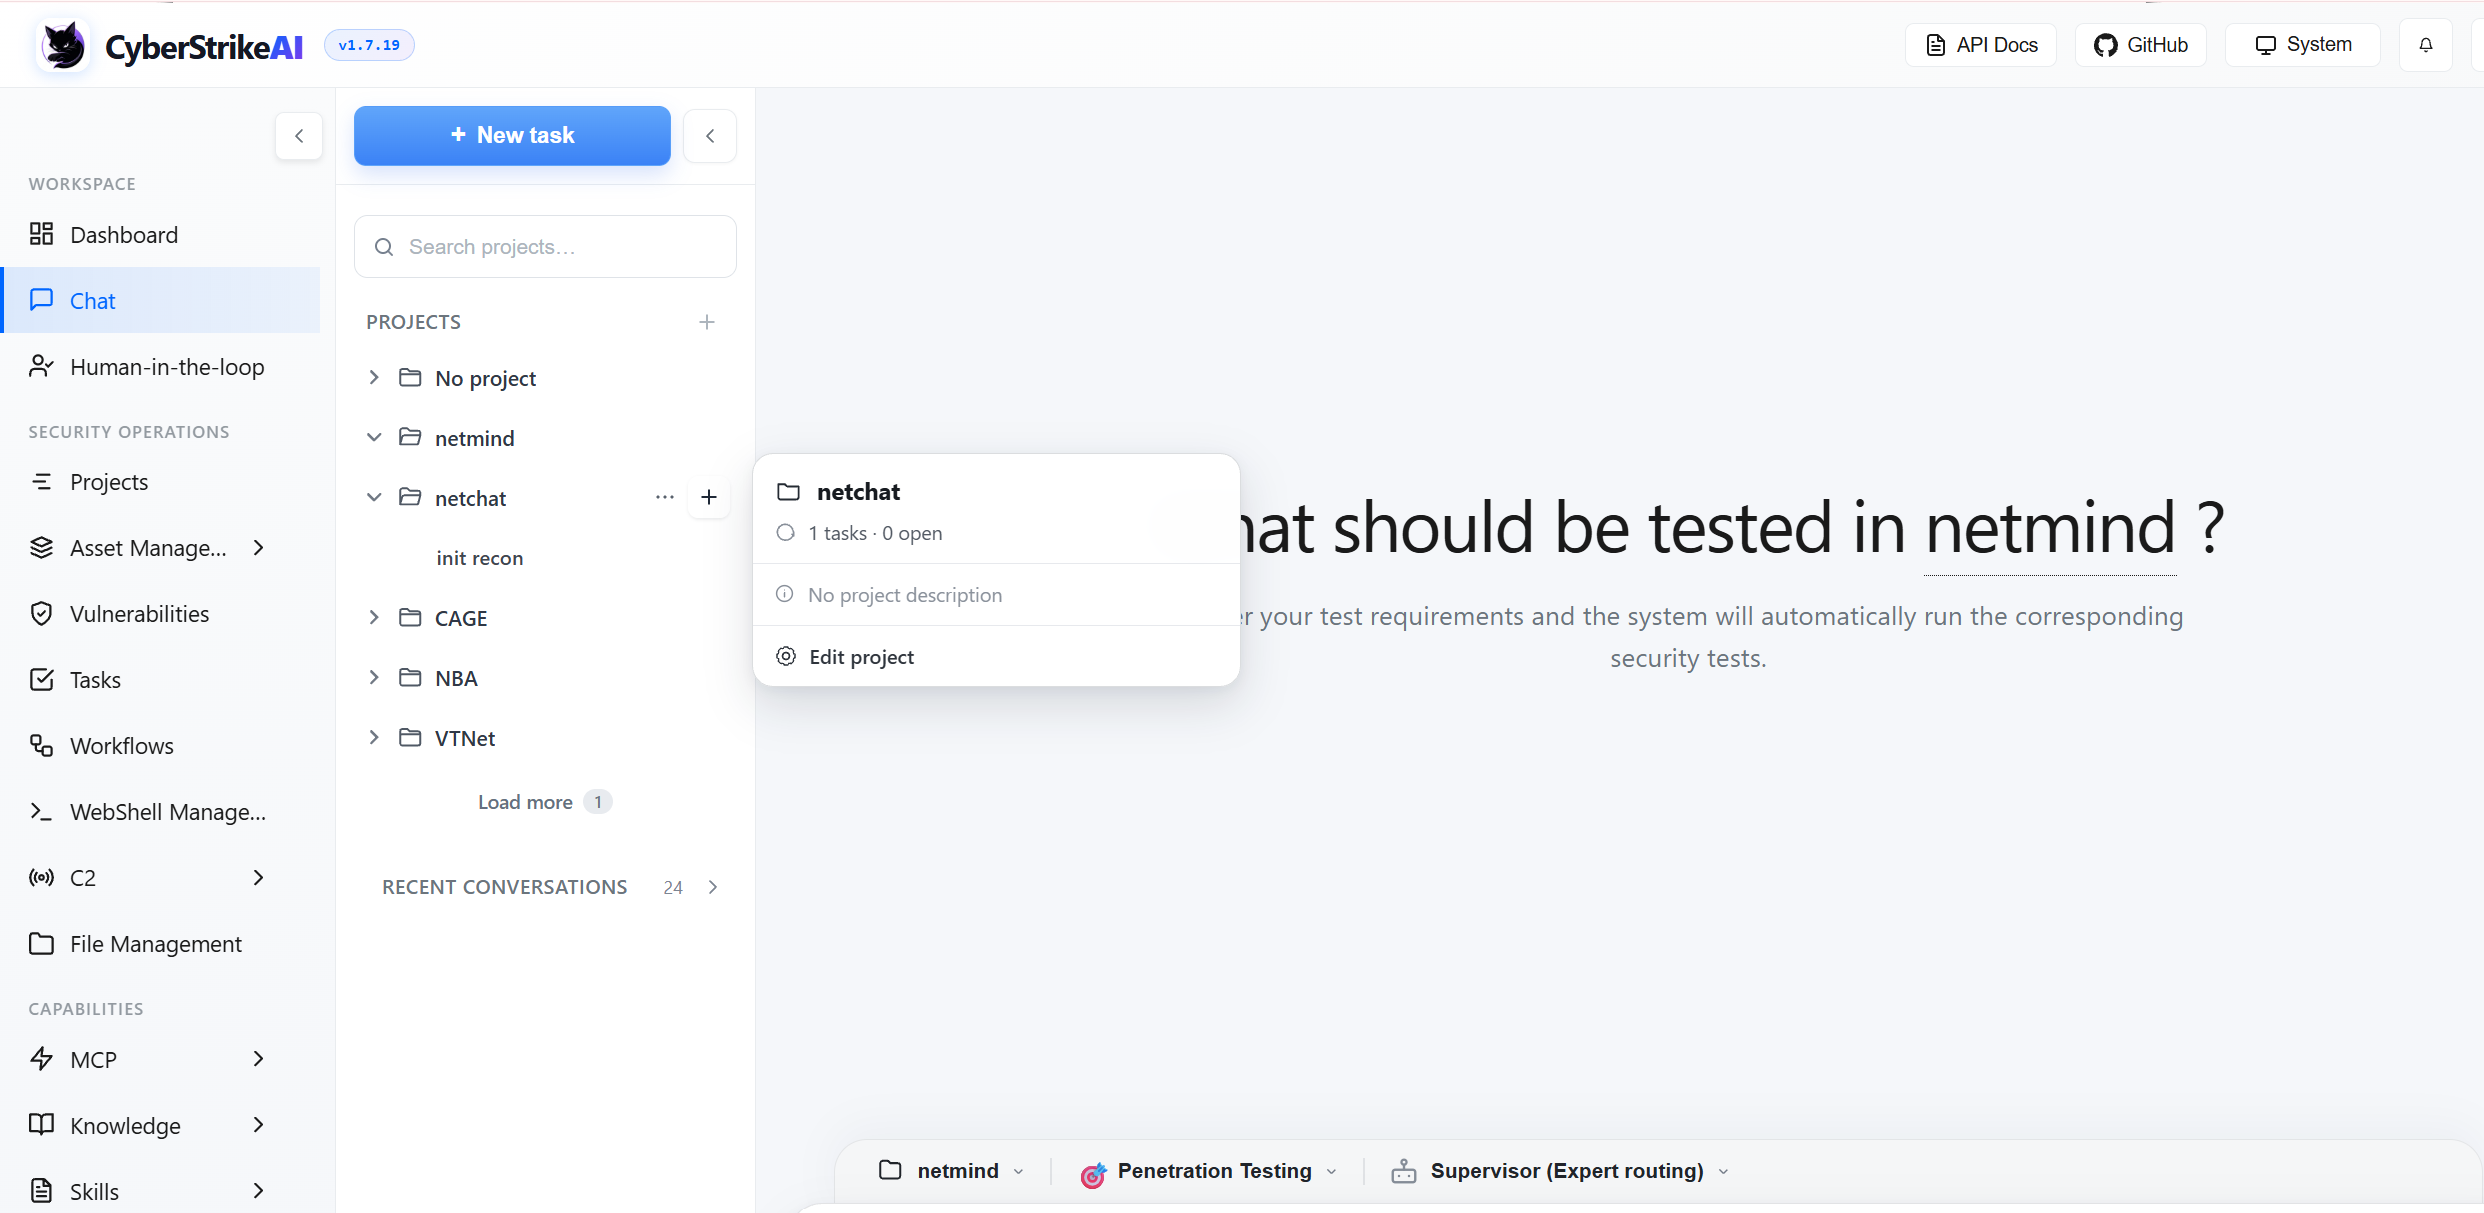
\includegraphics[width=0.66\textwidth,keepaspectratio]{02-chat-interface.png}
  \caption{Chat interface}
\end{figure}

\subsection{Bước 3: Chọn Role}

Click \textbf{Role selector} và chọn role phù hợp (vd \ccode{Penetration Testing}, \ccode{API Security Assessment}). Role định nghĩa \textbf{persona} (system prompt) và \textbf{tool scope} (công cụ được phép).

\subsection{Bước 4: Chọn Agent Mode}

Click \textbf{Agent mode selector} chọn chế độ: \ccode{eino\_single} (single agent), \ccode{deep} (task phức tạp), \ccode{plan\_execute} (Planner $\rightarrow$ Executor $\rightarrow$ Replanner), hoặc \ccode{supervisor} (điều phối sub-agents).

\begin{figure}[htbp]
  \centering
  \begin{minipage}{0.48\textwidth}
    \centering
    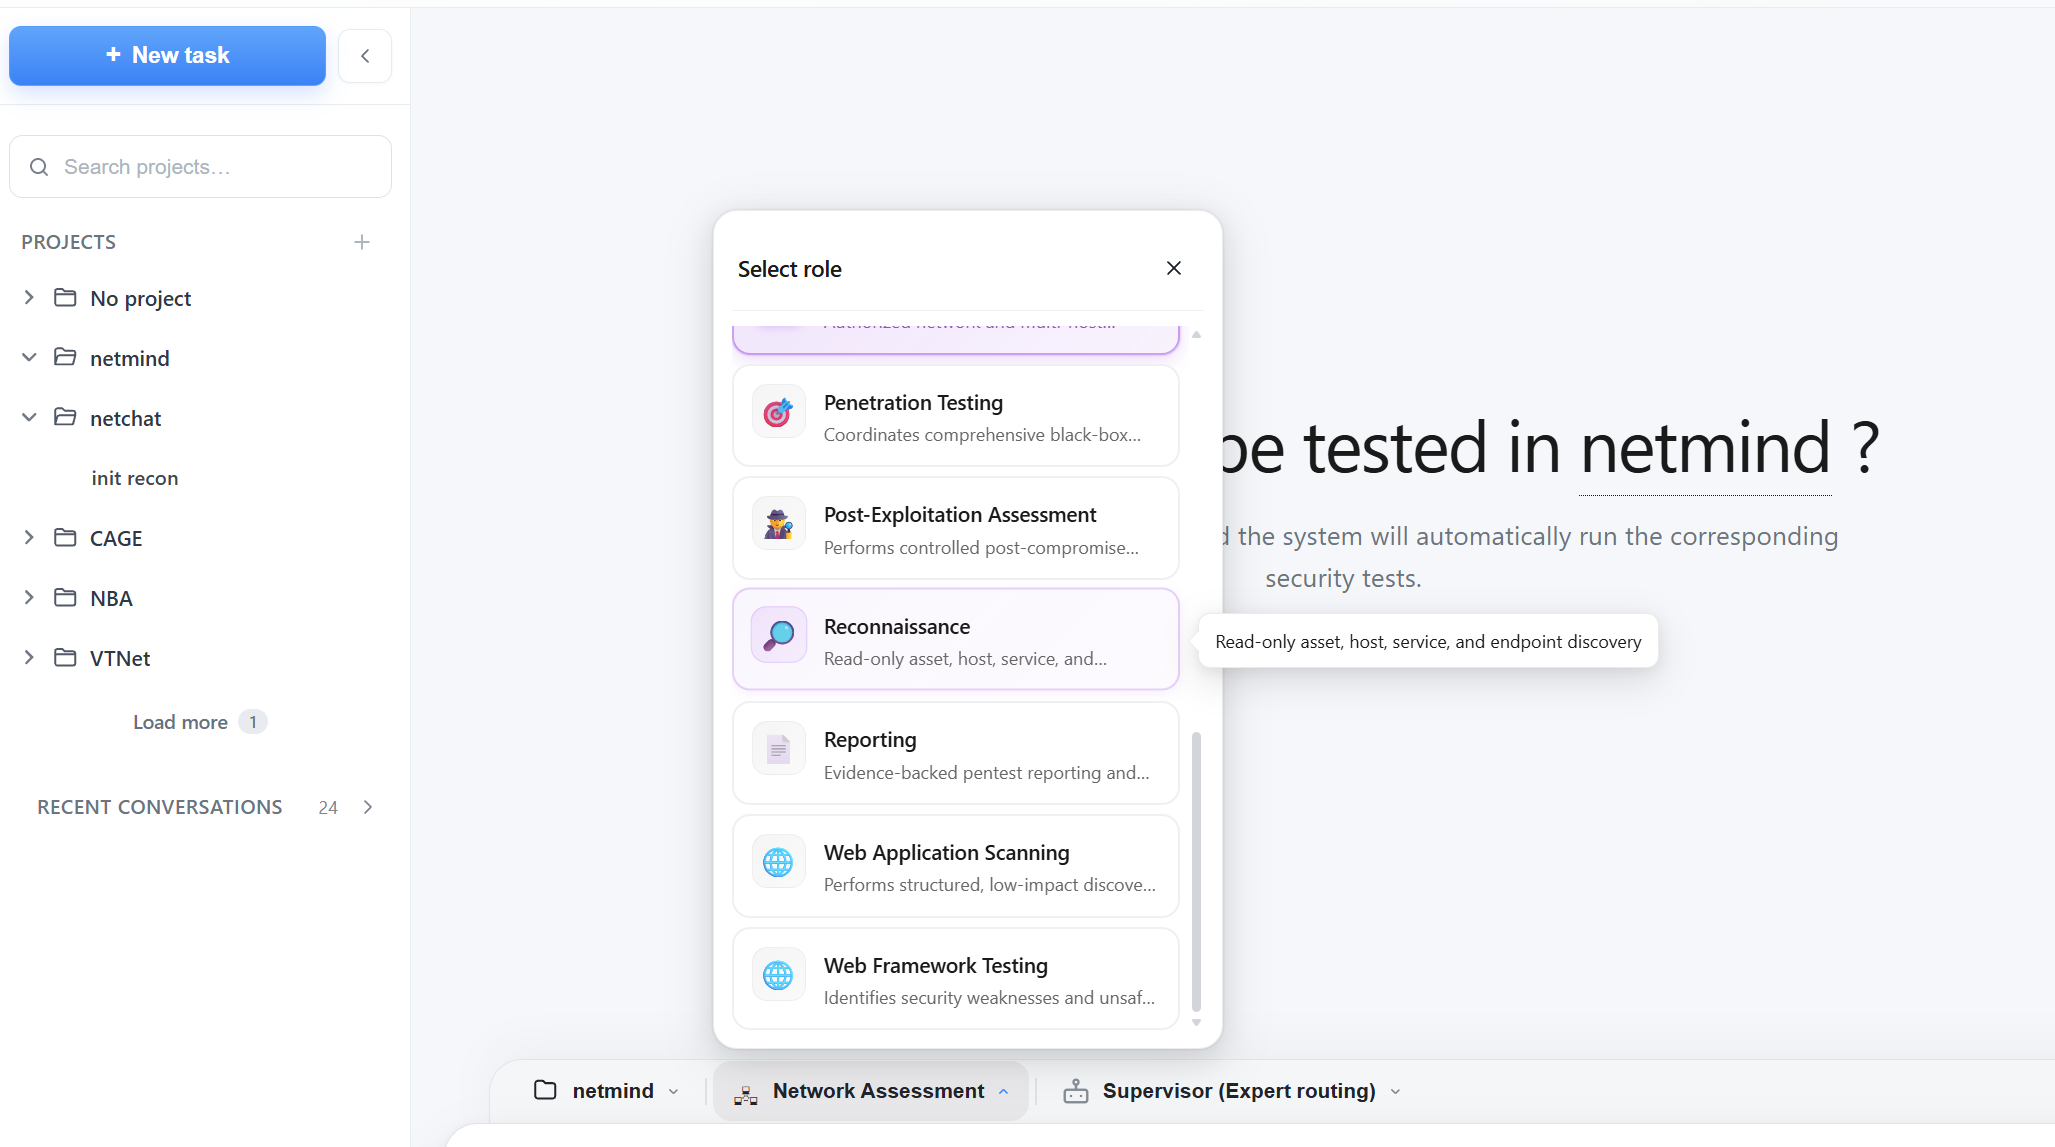
\includegraphics[width=\textwidth,keepaspectratio]{03-role-selector.png}
    \captionof{figure}{Role selector}
  \end{minipage}\hfill
  \begin{minipage}{0.48\textwidth}
    \centering
    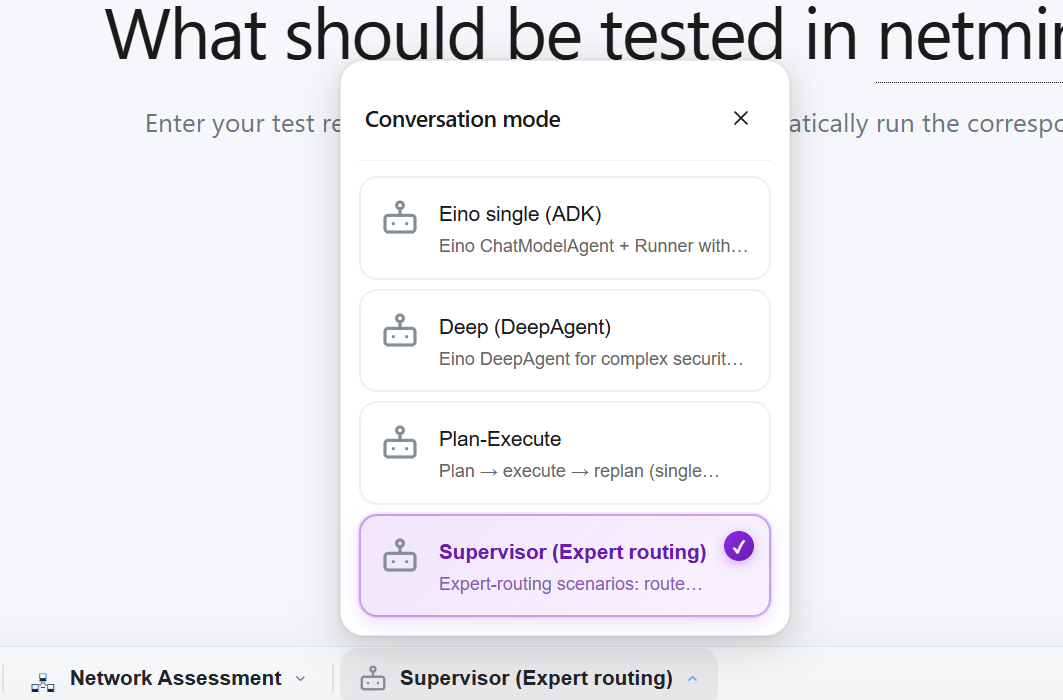
\includegraphics[width=\textwidth,keepaspectratio]{04-agent-mode.png}
    \captionof{figure}{Agent mode selector}
  \end{minipage}
\end{figure}

\subsection{Bước 5: Gửi Task}

Nhập yêu cầu trong composer rồi \textbf{Send} (hoặc Enter), ví dụ:

\begin{lstlisting}[]
Scan open ports on 192.168.1.1
Check if https://example.com/page?id=1 is vulnerable to SQL injection
Enumerate subdomains for example.com, then run nuclei against the results
\end{lstlisting}

\subsection{Bước 6: Theo dõi và Review Kết quả}

\textbf{Timeline} hiển thị tool calls, kết quả, execution trace, và số iterations. \textbf{Progress indicator} cho biết trạng thái đang chạy (elapsed), đợi phê duyệt HITL (countdown), hoặc hoàn thành (summary). Dùng nút \textbf{Stop} để hủy tác vụ đang chạy.

% ============================================================
% 4. Kết quả & Tính năng Nâng cao
% ============================================================
\section{Kết quả \& Tính năng Nâng cao}

\subsection{Quản lý Kết quả}

\begin{longtable}{L{3.2cm}p{12.3cm}}
  \toprule
  \textbf{Tab} & \textbf{Mục đích} \\
  \midrule
  \endhead
  \textbf{Facts} & Tri thức trích xuất từ chat (target, finding, chain), liên kết với vulnerability. Có \textbf{Key}, \textbf{Category} (target/finding/exploit/auth/infra/chain/poc/business/note), \textbf{Confidence} (tentative/confirmed/deprecated). \\
  \textbf{Assets} & Tài sản (host, domain, IP, service). Filter theo status/project/risk, batch actions (gán project, merge, export), import CSV/XLSX. \\
  \textbf{Vulnerabilities} & Lỗ hổng phát hiện. Card hiển thị severity, status, description, reproduction steps, evidence, impact, recommendation. Tạo từ fact (\textbf{Link} hoặc \textbf{Create vulnerability from fact}), export Markdown. \\
  \textbf{Tasks} & Tác vụ agent đang chạy/hoàn thành. Filter theo status, xem timeline/result/error. \\
  \bottomrule
\end{longtable}

\begin{figure}[htbp]
  \centering
  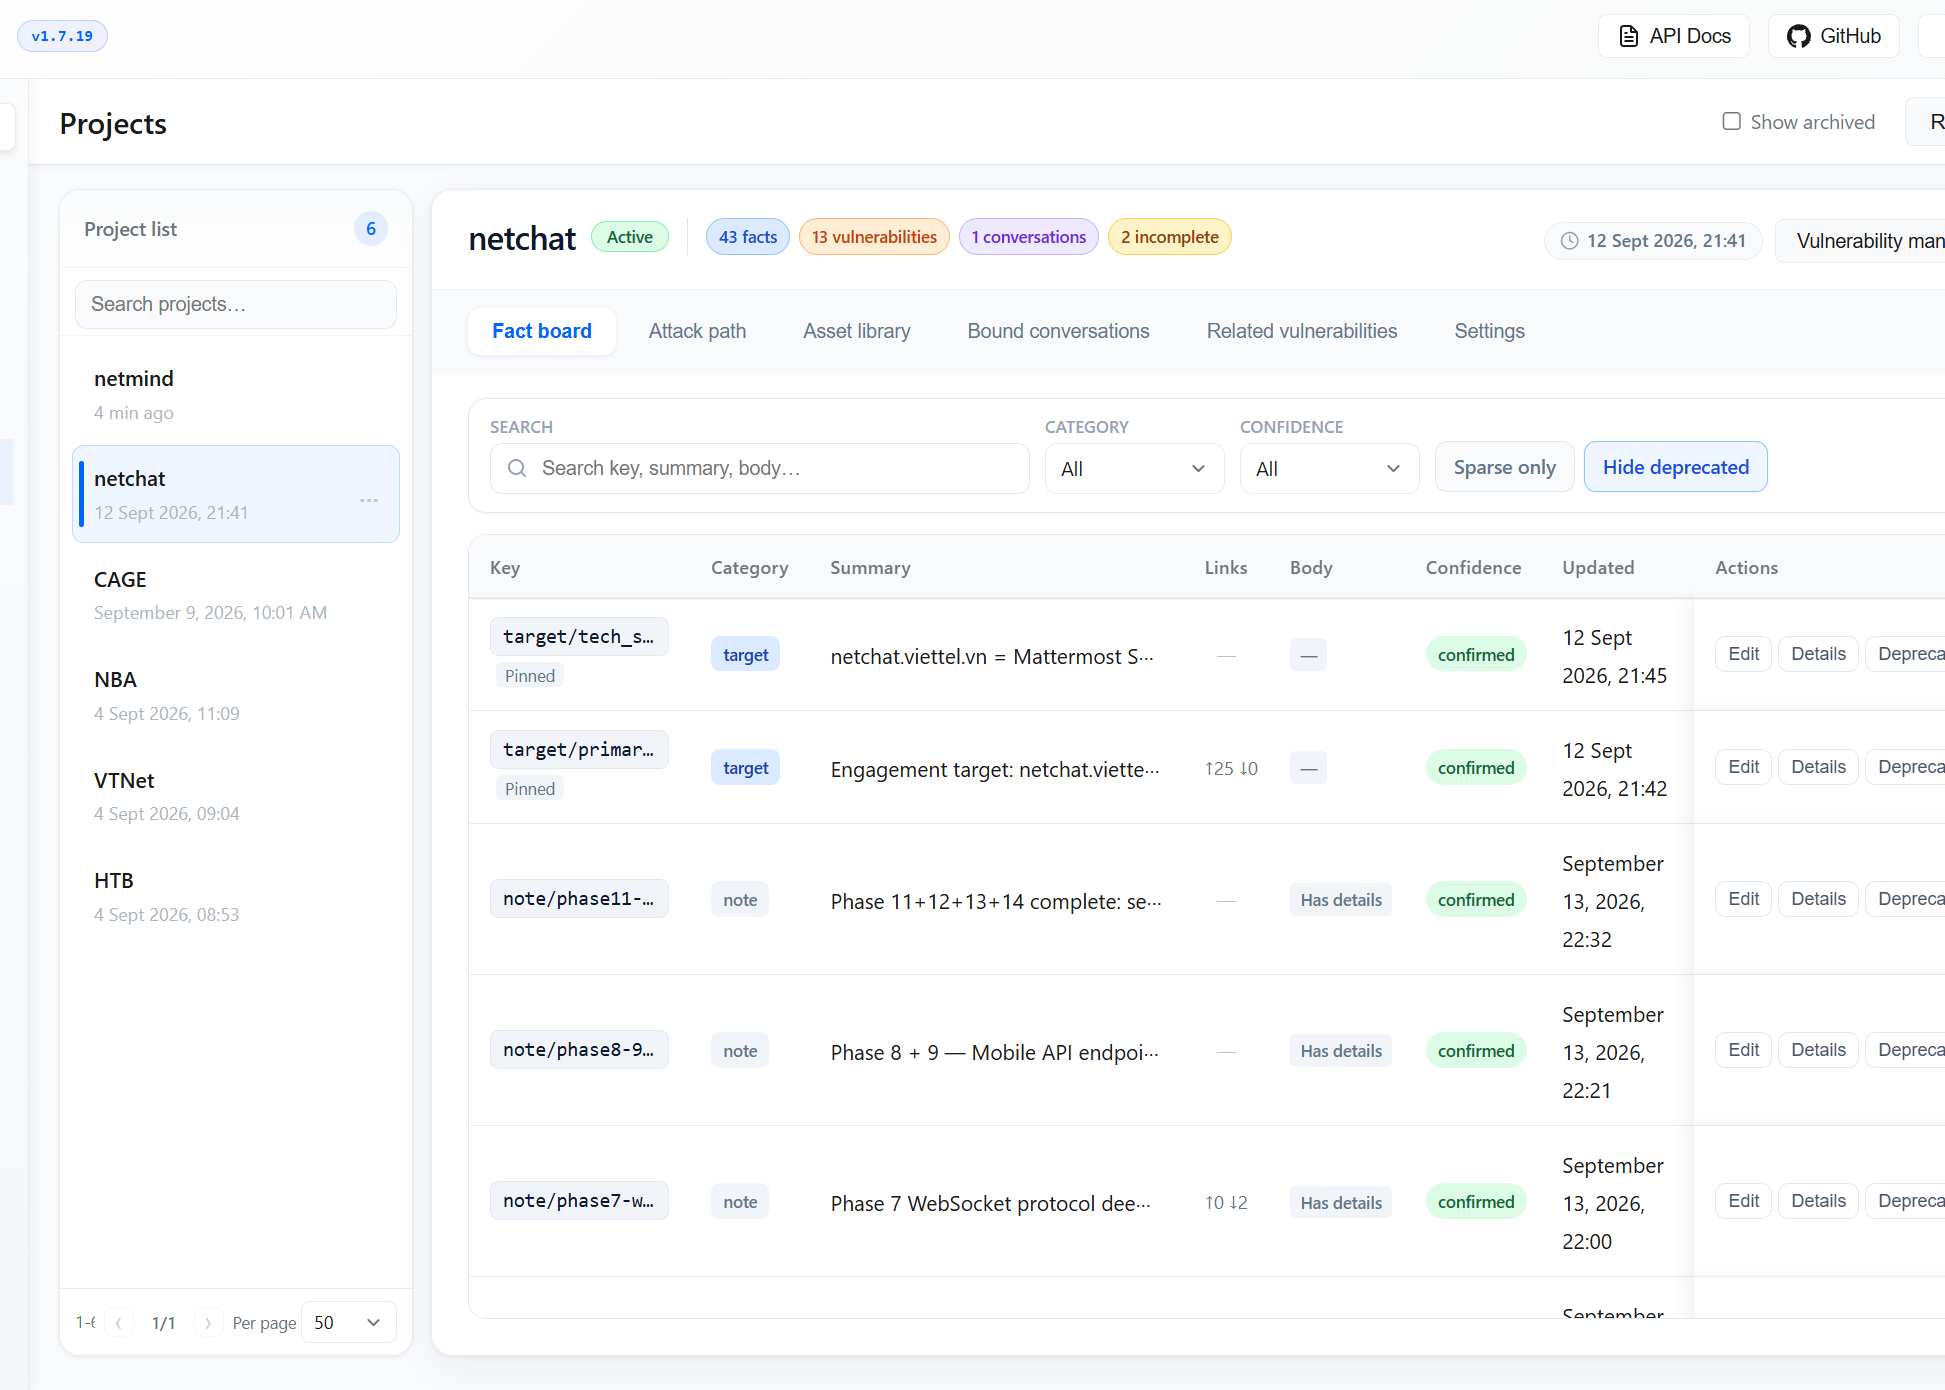
\includegraphics[width=0.72\textwidth,keepaspectratio]{01-facts_crop.png}
  \caption{Facts tab}
\end{figure}

\begin{figure}[htbp]
  \centering
  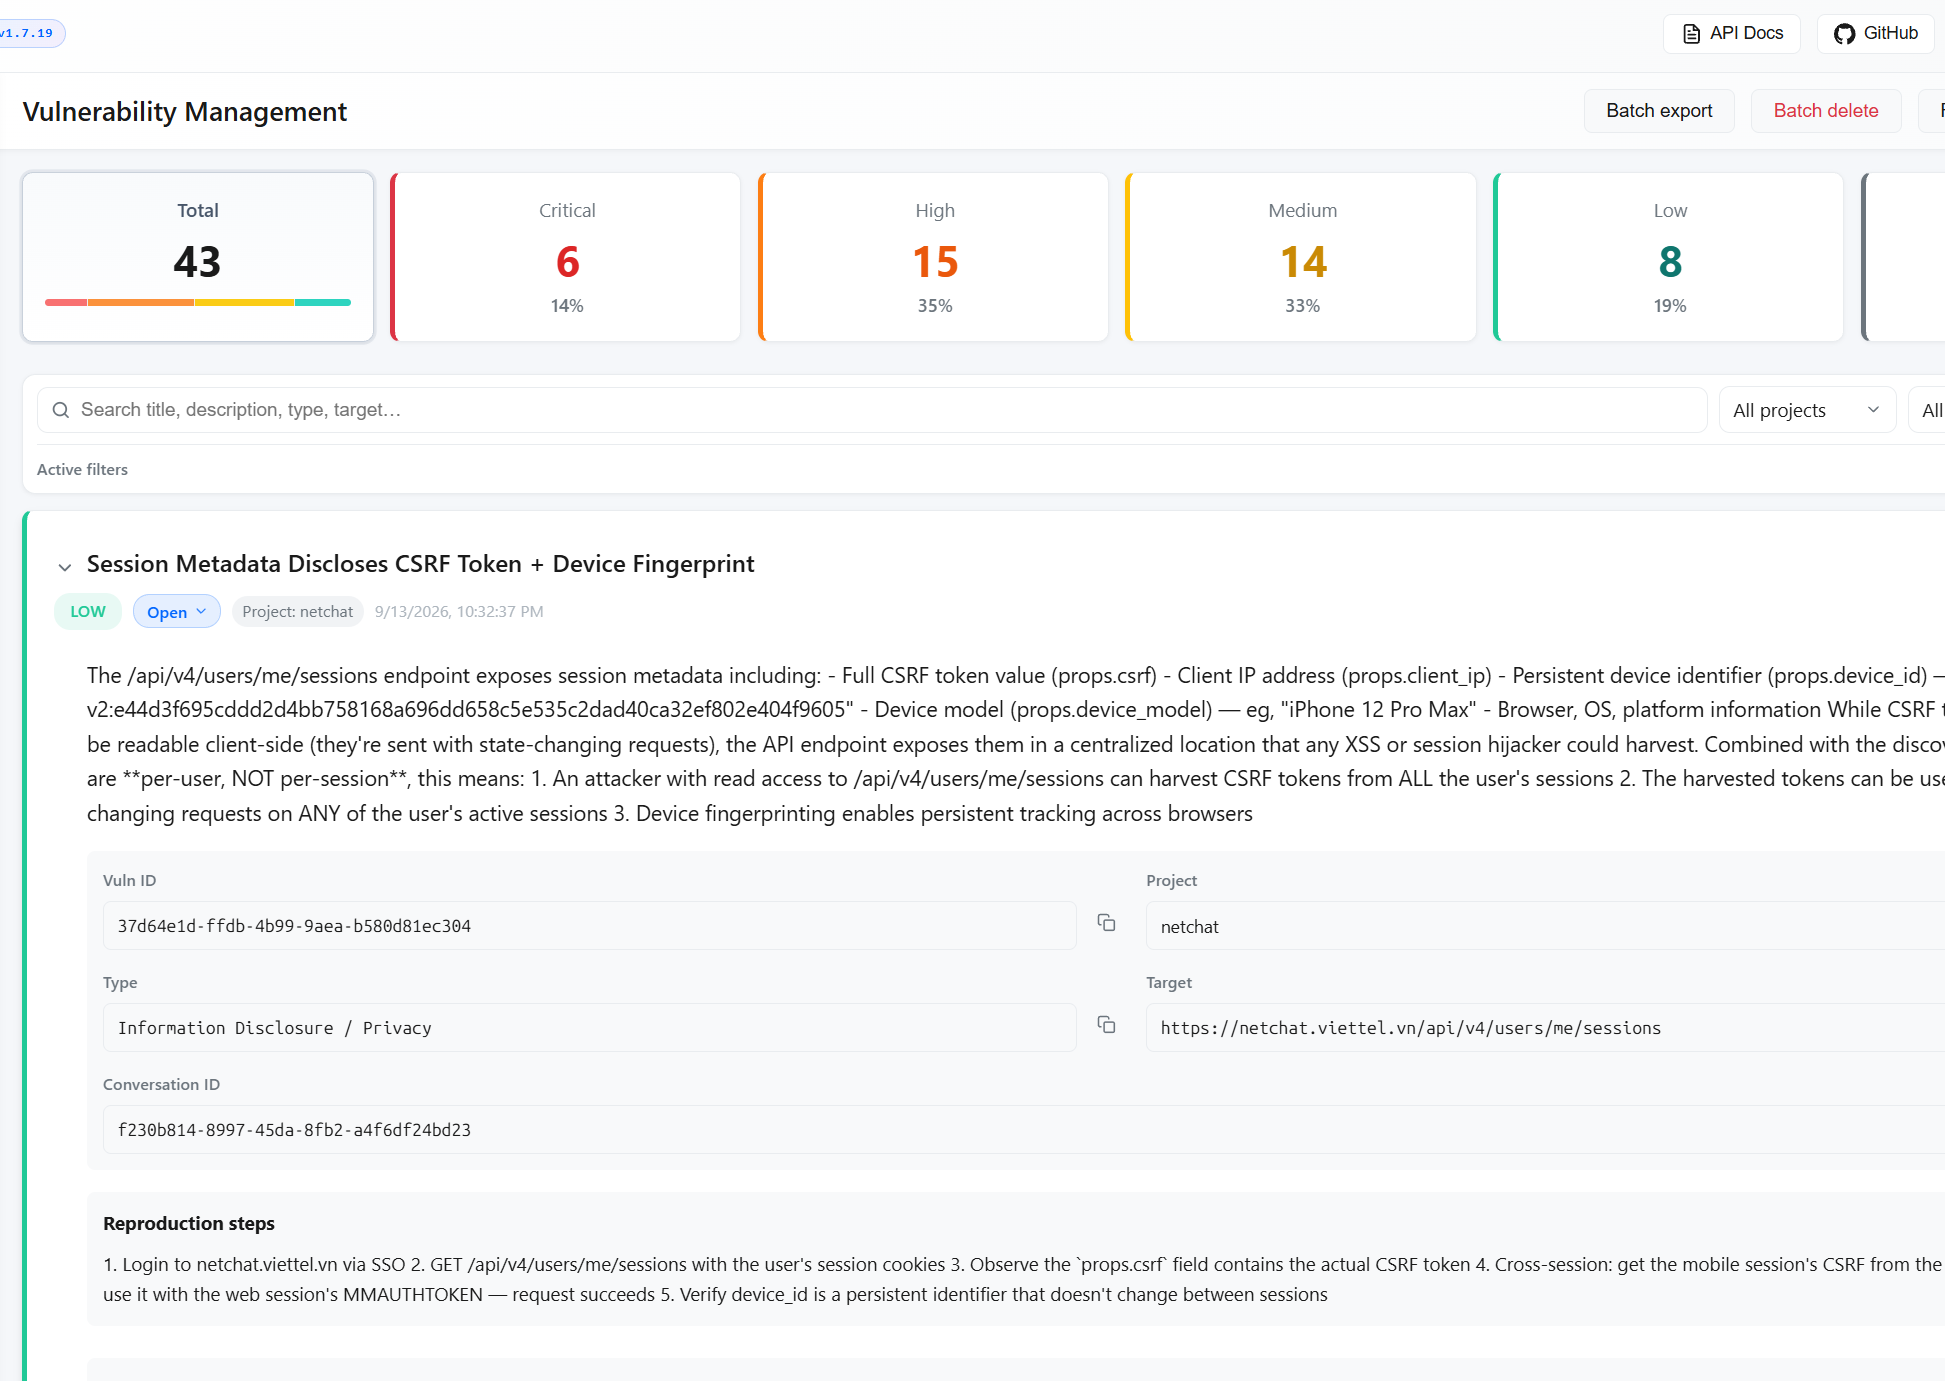
\includegraphics[width=0.72\textwidth,keepaspectratio]{03-vulnerabilities_crop.png}
  \caption{Vulnerabilities list}
\end{figure}

\subsection{Tính năng Nâng cao}

\textbf{Workflows} — đồ thị các node (start, tool, agent, condition, hitl, output, end) để tự động hóa tác vụ phức tạp. Hỗ trợ kéo-thả, \textbf{AI generate} (mô tả tự nhiên $\rightarrow$ draft graph), \textbf{Dry-run}, và export/import file \ccode{.csapkg.zip}.

\textbf{MCP (Model Context Protocol)} — dùng \textbf{MCP Monitor} để xem tool execution real-time (terminate/cancel) và \textbf{MCP Management} để thêm/xóa external servers, test connection. Tool MCP tự xuất hiện trong Chat khi kết nối thành công.

\textbf{Knowledge Base} — kho tri thức (tài liệu, CVE, best practices) để AI truy xuất (RAG). Thêm item, dùng \textbf{Scan} để phát hiện item mới, \textbf{Build Index} để tạo vector embeddings, và theo dõi qua \textbf{Retrieval Logs}.

\textbf{Skills} — gói kỹ năng (SKILL.md + script/file) cho agent. Theo dõi qua \textbf{Skills Monitor} (thống kê calls) hoặc CRUD trong \textbf{Management}. Trong Chat dùng tool \ccode{skill} để load.

\textbf{Agents} — sub-agents (multi-agent) định nghĩa bằng file Markdown trong \ccode{agents/}. \textbf{Orchestrator} là agent chủ điều phối, \textbf{Sub} là agent con thực thi; cấu hình gồm tools, max iterations, instruction.

\textbf{Roles} — persona (prompt + tool scope) cho agent. Chọn trong Chat thì tool list tự cập nhật; có thể tạo với name, icon, description, user prompt, tools, và enable/disable.

\textbf{Lưu ý:} \textbf{C2 (Command \& Control)} và \textbf{WebShell Management} là tính năng out-of-scope trong tài liệu này --- xem \ccode{docs/en-US/c2.md} và \ccode{docs/en-US/webshell.md}.

% ============================================================
% 5. Troubleshooting
% ============================================================
\section{Troubleshooting}

Dưới đây là các lỗi thường gặp theo định dạng \textbf{Vấn đề | Nguyên nhân | Cách xử lý}.

\begin{longtable}{L{3.6cm}L{4.6cm}p{7.3cm}}
  \toprule
  \textbf{Vấn đề} & \textbf{Nguyên nhân} & \textbf{Cách xử lý} \\
  \midrule
  \endhead
  \ccode{Failed to load config} & \ccode{config.yaml} không tồn tại hoặc lỗi YAML. & Kiểm tra file tồn tại. Validate: \ccode{python3 -c "import yaml; yaml.safe\_load(open('config.yaml'))"}. \\
  \ccode{Failed to open database} & \ccode{data/} không ghi được hoặc DB corrupt. & Kiểm tra quyền ghi \ccode{data/}. Backup \& xóa \ccode{data/conversations.db} để reset. \\
  \ccode{port already in use} & Port 7123/7134 đã bị chiếm. & Đổi port trong \ccode{config.yaml} (\ccode{server.port}, \ccode{mcp.port}). \\
  \ccode{401 Unauthorized} & API key sai/thiếu. & Kiểm tra \ccode{ai.channels.<id>.api\_key} trong \ccode{config.yaml}. \\
  \ccode{404 Not Found} & Base URL sai. & Kiểm tra \ccode{base\_url} (phải có \ccode{/v1} path cho OpenAI-compatible). \\
  \ccode{Rate limit} & Vượt quota API. & Chờ hoặc nâng gói API. \\
  \ccode{Model not found} & Model name sai. & Kiểm tra model name (vd \ccode{MiniMax/MiniMax-M3}, \ccode{gpt-4o}). \\
  Tool chưa cài & Công cụ chưa có trong PATH. & Cài tool: \ccode{sudo apt install nmap sqlmap gobuster}. \\
  Tool YAML lỗi & File \ccode{.yaml} trong \ccode{tools/} có lỗi cú pháp. & Kiểm tra YAML syntax; restart server để reload. \\
  Role không có tool & Role bị giới hạn tool scope. & Edit role $\rightarrow$ Thêm tool vào danh sách. \\
  \ccode{mcp.enabled: false} & MCP chưa bật trong config. & Set \ccode{mcp.enabled: true} trong \ccode{config.yaml}. \\
  Port conflict (MCP) & Port 7134 đã dùng. & Đổi \ccode{mcp.port} trong config. \\
  External MCP không kết nối & URL/command sai. & Kiểm tra \ccode{external\_mcp.servers}; click \textbf{Test connection} trong MCP Management. \\
  \ccode{max\_iterations} reached & Agent lặp quá nhiều vòng. & Tăng \ccode{agent.max\_iterations} trong config hoặc kiểm tra prompt. \\
  Tool timeout & Tool chạy quá lâu. & Tăng \ccode{agent.tool\_timeout\_minutes} trong config. \\
  HITL pending & Đợi phê duyệt. & Vào \textbf{Human-in-the-loop} $\rightarrow$ Approve/Reject. \\
  Model error & Model trả về sai định dạng. & Kiểm tra model response trong log; đổi model/channel. \\
  \bottomrule
\end{longtable}

\textbf{Kiểm tra logs bổ sung:} dùng Terminal (server log), \textbf{System Settings $\rightarrow$ Audit Logs} (thao tác người dùng), \textbf{MCP Monitor} (tool execution). Test kết nối model qua \textbf{System Settings $\rightarrow$ AI Channel Configuration $\rightarrow$ Test connection}.

Nếu vẫn gặp vấn đề, xem \ccode{docs/en-US/troubleshooting.md} và \ccode{docs/en-US/configuration.md}, hoặc mở issue tại \url{https://github.com/Ed1s0nZ/CyberStrikeAI/issues}.

\end{document}
